\section{Data Analysis}
\label{sec:analysis}

This analysis is performed using XENON100 Run-II science data, with 224.6~live days of data taking. The detector's response to ERs has been characterized with $^{60}$Co and $^{232}$Th calibration sources, while the response to NRs was calibrated with an $^{241}$AmBe $(\alpha,n)$-source. This fast neutron source gives rise to elastic and inelastic neutron-nucleus scatters, and can thus be employed to define the expected signal region for inelastic WIMP-nucleus scatters.


\begin{figure*}[t!]
	\begin{subfigure}{0.49\linewidth}
		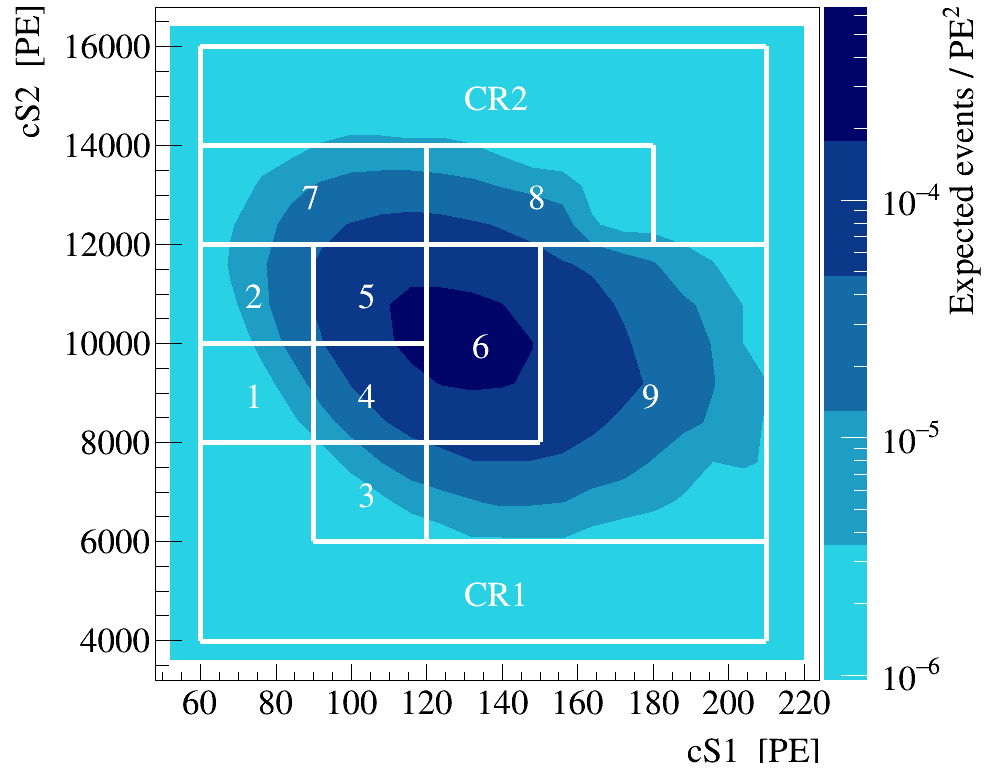
\includegraphics[width=\linewidth]{images/wimp_in_sr.png}
		\subcaption{}
	\end{subfigure}
	\begin{subfigure}{0.49\linewidth}
		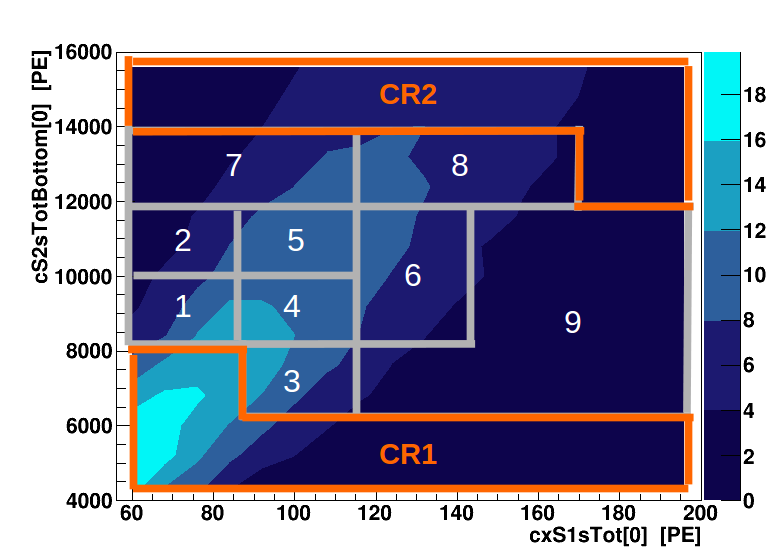
\includegraphics[width=\linewidth]{images/bkg_in_sr.png}
		\subcaption{}
	\end{subfigure}
	\caption{\raggedright Signal (1-9) and control (CR1 and CR2) regions for the inelastic WIMP-$^{129}$Xe interaction in the (cS2,cS1)-plane.
		\textcolor{red}{Figure (a) shows the signal distribution for a simulated WIMP of mass 100\,GeV/c$^2$, while Figure (b) is obtained using  $^{60}$Co calibration data 
	and represent the background expectation distribution.}}
  \label{fig:SR}
\end{figure*}

\subsection{Signal Correction} 

A particle interaction in the liquid xenon produces an S1 and a correlated S2 signal with a certain number of photoelectrons (PE) observed by the PMTs. The non-uniform scintillation light collection by the PMT arrays, due to solid angle effects, Rayleigh scattering length, reflectivity, transmission of the electrodes, etc, lead to a position-dependent S1 signal. The warping of the top meshes (inducing a variation in the width of the gas gap between the anode and the liquid-gas interface), the absorption of electrons by residual impurities as they drift towards the gas region, as well as solid angle effects lead to a position-dependent S2 signal. These signals are thus corrected in 3 dimensions, using various calibration data, as detailed in~\cite{Aprile:2011dd,Aprile:2012vw}, with the corrected quantities denoted as cS1 and cS2, and defined in~\cite{Aprile:2012vw}. 
%The trigger efficiency in this run was 100\% for S2$>$300\,PE.

\subsection{Signal Region and Event Selection} 

As explained in Section~\ref{sec:intro}, the inelastic scattering of a WIMP with a $^{129}$Xe nucleus is expected to produce an energy deposit via a NR with subsequent emission of  
a 39.6\,keV de-excitation photon. The largest fraction of the energy released in the event is via an ER, due to the emitted photon which loses its energy in the LXe.
This represents an unusual signature compared to the one expected from an elastic scatter, and brings the signal region to overlap with the ER background region.
%{\textcolor{red} {Should we mention that AmBe data is used here, to define these regions? And should we provide somewhere the used energy ranges in cS1 and cS2?}}
The selected region of interest (ROI) for this analysis surrounds the 39.6\,keV xenon line in the (cS1,cS2)-plane 
\textcolor{red} {and is based on $^{124}$AmBe calibration data, it extends from 60 to 200\,PE in cS1 and from 4$\times \, 10^3$ to 16$\times \, 10^3$\,PE in cS2, it is further divided  into sub-regions}
\sout{and is further divided into sub-regions,} as shown 
in Figure~\ref{fig:SR}.  These sub-regions were defined such as to roughly contain a similar number of expected background events in each region. The control regions (denoted as CR1 and CR2 in the figures), are selected to be as close as possible to the signal regions,  and are used for cross checks of the background shape distribution.

Apart from the condition to occur in the defined region of interest in the (cS1,cS2)-plane, valid events are required to fulfil several selection criteria, 
which can be summarized as follows: basic data quality cuts, energy selection and S2 threshold cut, veto cut for events with energy release in the detector's active LXe shield, 
selection of single-scatter events and of a predefined fiducial volume 
\textcolor{red}{of 34\,kg}.  
Our analysis closely follows the event selection criteria described in detail in \cite{Aprile:2012vw} for Run-II, with only a few exceptions, as explained in the following. 
The cut on the width of the S2 signal as a function of drift time (where the maximal drift time is 176\,$\mu$s and the width values range from $\sim$1-2\,$\mu$s) has been optimized on a sample of events selected from the 39.6\,keV line and set to a 95\% acceptance on these. This cut ensures that the S2-signal width is consistent with the $z$-position calculated from the observed time difference between the S1 and S2 signals. Events are required to be single-scatters by applying a threshold cut on the size of the 
second largest S2 peak. For this analysis, the threshold has been optimized to 160\,PE and set constant as function of S2 signal size. 
\sout{Finally, the chosen fiducial volume corresponds to 34\,kg of liquid xenon, which is identical to the one used for the elastic scattering channel~\cite{Aprile:2012vw}}. 





\subsection{Signal Simulation} 

The detector response to inelastic WIMP-$^{129}$Xe interactions was simulated using an empirical signal model.
The total deposited energy is divided into two independent contributions: one coming from the 39.6\,keV de-excitation photon and the other  from  
the simultaneous nuclear recoil of the xenon atom. The detected light (S1) and charge (S2) signals are simulated separately for each of the two contributions 
and then added together. This recipe has been followed  because the light and charge yields depend both on the type of interaction (ER vs. NR), and on the deposited energy.


The distribution of an ER induced by the de-excitation photon in the (cS1,cS2)-plane  is simulated assuming a two dimensional normal probability distribution function (pdf), $f(cS1_{er},cS2_{er})$, 
described (apart from a constant normalization factor) by the following equation:

\begin{multline}
	f(cS1_{er},cS2_{er})  = {\rm exp} \Big\{ -\frac{1}{2(1-\rho^2)} \Big[ \frac{(cS1_{er} - \mu_{cS1})^2}{\sigma_{cs1}^2} + \\ 
	 \frac{(cS2_{er} - \mu_{cS2})^2}{\sigma_{cs2}^2} - \frac{2\rho\cdot(cS1_{er} - \mu_{cs1}) (cS2_{er} - \mu_{cs2})} {\sigma_{cs1}\sigma_{cs2}} \Big] \Big\}
	%f(cS1,cS2) ~ = ~  \frac{1}{2 \pi \sigma_{cs1} \sigma_cs2 \sqrt{1-\rho^{2}} } exp \Big( -\frac{1}{2(1-\rho^2)} \Big[ \frac{(cS1 - \hat{cS1})^2}{\sigma_{cs1}^2} \Big] \Big)
\label{f:2dgaus}
\end{multline}
where $\mu_{cS1}$ and $\mu_{cS2}$ 
represent the average observed $cS1_{er}$ and $cS2_{er}$ signals given a 39.6\,keV ER, $\sigma_{cs1}$ and $\sigma_{cs2}$ are the standard deviation in $cS1_{er}$ and $cS2_{er}$ respectively,
while $\rho$ stands for the correlation between the cS1 and cS2 signals. The detector-related light yield $L_y$  at 39.6\,keV, necessary to evaluate the average number of prompt photons detected 
($\mu_{cS1}$), is obtained from the NEST model~\cite{NEST,Geant1,Geant2} fit to data collected with several $\gamma$-lines.
%%%%% REMOVEME %%%%%%
\sout{The average light yield at 39.6\,keV is 2.7\,PE/keV.}

The same model is used to predict the charge yield at 39.6\,keV, which is then scaled according to the detector's secondary scintillation gain $Y$. 
 The latter is determined from detector's response to single electrons~\cite{SingleE}.
The energy resolution at 39.6\,keV in cS1 and cS2 has been measured to be 15.8\% and 14.7\%, respectively, and is used to extract the standard 
deviations $\sigma_{cs1}$, $\sigma_{cs2}$.  The correlation parameter is assumed to be independent of energy (at least in the considered narrow energy range) and measured
using the 164\,keV line from the decay of the $^{131m}$Xe isomer ($T_{1/2}$=11.8\,d) produced during the  $^{124}$AmBe run. This $\gamma$-line is chosen because it allows to disentangle efficiently the contribution from the nuclear recoil. The measured correlation coefficient is $\rho \, = \, -0.45 \pm 0.10$. 


The cS1 and cS2 distributions from the NR contribution are predicted starting from the expected nuclear recoil energy spectrum
of WIMP inelastic interactions~\cite{Baudis:2013bba}. The average cS1 and cS2 are given by equations~\ref{f:cs1} and~\ref{f:cs2} respectively,
where $\mathcal{L}_{eff}$ is the liquid xenon relative scintillation efficiency for NRs, while $S_{ee} \, = \, 0.58$  and $S_{nr} \, = \, 0.95$ describe the scintillation 
quenching  of ER and NRs, respectively, due to the electric field \cite{ScintQuenching}. The parameterization and uncertainties of $\mathcal{L}_{eff}$ as a function of nuclear recoil energy $E_{nr}$ are based on existing 
direct measurements \cite{run8Result}. The light yield for 122\,keV ERs is taken from the same NEST model fit as described above. For cS2, the parameterization 
of $Q_{Y}(E_{nr})$ is taken from \cite{QY}. Finally, all detector related resolution effects are introduced following the prescriptions described in \cite{Aprile:2012vw}.

\begin{equation}
cS1_{nr} ~=~ E_{nr} \, \mathcal{L}_{eff}(E_{nr}) \, L_{y} \, \frac{S_{nr}}{S_{ee}}
\label{f:cs1}
\end{equation}

\begin{equation}
cS2_{nr}  ~ = ~ E_{nr} \, Q_{Y}(E_{nr}) \, Y
\label{f:cs2}
\end{equation}

%%%%% DEPENDING ON if we add it before %%%%%
%{\textcolor{red} {Should we also give the numerical values of $L_Y$ and $Y$?}}
The pdf of the ER and NR contributions are then convoluted together to obtain the overall pdf of the expected signal.
A 2D (cS1 versus cS2) acceptance map is applied to the signal pdf to reproduce data selection effects. Acceptances are computed separately for each selection 
criteria using the $^{124}$AmBe calibration sample. \textcolor{red}{Acceptances of} other selections such as the liquid xenon veto cut, and the single-scatter interaction represent an exception  and 
a dedicated computation has been performed in these cases. The combined acceptance  of all selection criteria in the region of interest averages to $\sim$$(0.80\pm0.05)$. 
Figure~\ref{fig:unc} shows an example of fully simulated signal model for a WIMP mass of 100\,GeV/c$^2$. 

The signal simulation procedure has been validated by reproducing the 39.6\,keV xenon line from interactions due to neutrons from the 
$^{124}$AmBe source and compared to data. For this comparison, the  $^{124}$AmBe nuclear recoil interactions and their acceptances
were simulated. The simulated events were in agreement  with calibration data within statistical uncertainties. 
%%%%%% DEPENDS on the journal  %%%%%
%{\textcolor{red} {Should we show an example, namely a figure from the signal model note?}}



\subsection {Background Model}

The background in the region of interest for inelastic scattering is dominated by ERs due to the residual radioactivity of detector materials, due to $^{85}$Kr present in the liquid xenon ($\sim$55\%) as well as due to $^{222}$Rn decays in the liquid ($<$7\%)~\cite{Aprile:2011vb}. The background contribution from inelastic scatters of radiogenic or cosmogenic neutrons (producing a 39.6\,keV de-excitation line) is negligible thanks to the very low expected neutron scattering rate in the detector~\cite{Aprile:2013tov}.


The expected background is modelled using data from the $^{60}$Co calibration campaign, which are assumed to well represent the background density distribution 
in the (cS1,cS2)-plane. The calibration sample yields  about $2.2\times10^4$ events in the ROI; these are then scaled to the science data according to a measured scale 
factor $\tau_{bkg}$. This scale factor, which is merely the ratio between the data and calibration sample yields, is measured in the two control regions shown in Figure~\ref{fig:SR} (labelled CR1 and CR2) separately. The two control regions give compatible results and the computed average is $\tau_{bkg} \, =  \, 0.034 \pm 0.002 $, where the reported uncertainty 
is of statistical nature only.

The distribution of the calibration sample has been compared to the data of the science run in the two control regions,
and agreement was found within statistical uncertainties. Furthermore, $^{60}$Co calibration data have been compared in the region of interest to  
data from the $^{232}$Th calibration campaign, and the largest deviation between the two shapes is within 4\%. 
%%%%% Said later anyway, propose to remove it here %%%%%
\sout{An additional systematic uncertainty of 4\% has thus been applied to the expected background yield of each sub-region of the ROI.}

%%%%%% DEPENDS on the journal  %%%%%
%{\textcolor{red} {Should we show a figure, namely the agreement of data and BG model for the control regions? Like the second figure in the background model check note.}}



\subsection{Systematic Uncertainties}

\begin{figure}[t!]
  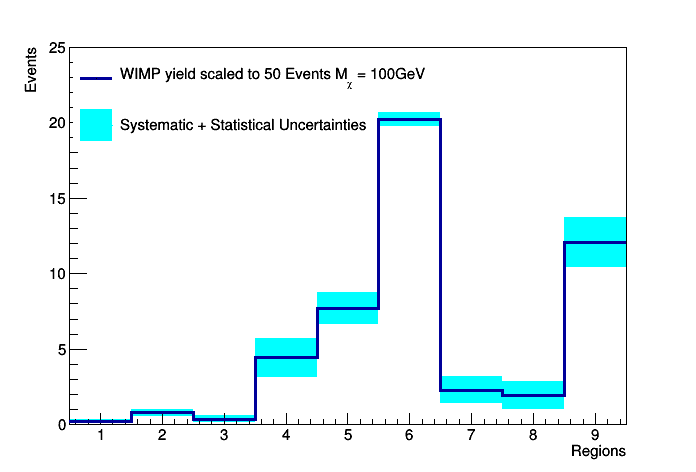
\includegraphics[width=\linewidth]{images/wimp_sys_unc.png}
  \caption{Predicted signal \textcolor{red} {yield in each sub-region} (blue curve), along with statistical and systematic uncertainties (cyan area) simulated for a WIMP mass of 100\,GeV/c$^2$.  
	   The signal has been scaled for a total number of 50 events. }
  \label{fig:unc}
\end{figure}


Uncertainties on the  prediction of the total number of background events arise from the uncertainty on the measurement of the normalisation 
factor, $\tau_{bkg}$, and amount to 6\%. % contribution of radiogenic neutrons are neglected. 
Systematic uncertainty on the shape of the predicted background distribution are assessed by the maximal observed discrepancy in the ROI between
the $^{60}$Co and $^{232}$Th calibration samples.  
\sout{As explained} A 4\% systematic uncertainty is added  to the expected yield of each sub-region.
Uncertainties belonging to different sub-regions in the ROI are considered independent from one another.

Uncertainties on the total yield of signal events arising from selections acceptance uncertainties are found to be very weakly dependent on 
the WIMP mass, and an overall 6\% acceptance uncertainty is applied to all WIMP hypotheses. 

Uncertainties on the energy scale and, more generally, related to detector responses  are parameterised 
using the respective uncertainties on the measures of $L_y$, $\mathcal{L}_{eff}$, $Y$, $Q_Y$ and $\rho$. The simulation shows 
that these uncertainties mainly affect the pdf of the signal model in the ROI, and very weakly the total signal yield. 
They are taken into account by simulating several signal pseudo-samples for each WIMP mass, where the pseudo-samples are produced 
by varying the model parameters within their $\pm 1$ standard deviations. 
For each sub-region an overall uncertainty is then computed, by adding in quadrature the variations of each pseudo-sample 
with respect to nominal. Figure~\ref{fig:unc} shows an example of such a systematic uncertainty computation for a WIMP mass of 100\,GeV/c$^2$.


All the uncertainties discussed here are parameterised 
\sout{with}  \textcolor{red}{within} 
a binned profile likelihood function using the \textcolor{red}{ROOSTAT-ROOFIT framework}~\cite{roostat,roofit}.
\sout{using the framework from}~\cite{roostat,roofit}.
All the parameters related to systematic uncertainties are assumed to be normally distributed.


















